\documentclass{article}

\usepackage{stmaryrd}
\usepackage{amssymb}
\usepackage{tikz}
\usetikzlibrary{positioning}
 
\title{Interaction Diagram - Edit Author Description}
\author{ Steve Monson }

% no page number at bottom
\pagenumbering{gobble}

\begin{document}
\maketitle

\begin{center}

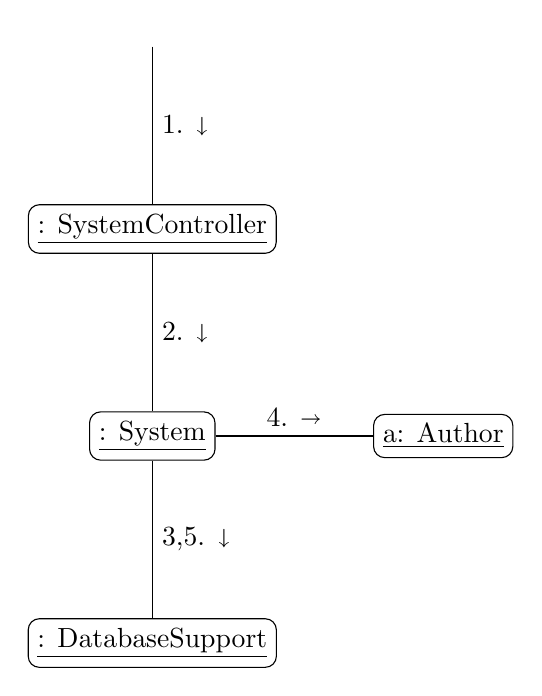
\begin{tikzpicture}[
  auto,
  block/.style = {
    rectangle,
    draw=black,
    align=center,
    rounded corners
  },
  multiple/.style = {
    rectangle, draw, rounded corners, fill= white,
    text width=9em, align= center,
    copy shadow = {
      ,fill=white, draw=black,
      shadow xshift=0.5mm, shadow yshift=-0.5mm
    }
  }
]
\node[] (start)  {};

\node[block, below = 2cm of start]      (controller) {\underline{: SystemController}};
\node[block, below = 2cm of controller] (system)     {\underline{: System}}; 
\node[block, below = 2cm of system]     (database)   {\underline{: DatabaseSupport}};
\node[block, right = 2cm of system]       (author)       {\underline{a: Author}};

\draw (start)      -- (controller) node[midway] {1. $\shortdownarrow$};
\draw (controller) -- (system)     node[midway] {2. $\shortdownarrow$};
\draw (system) -- (database)        node[midway] {3,5. $\shortdownarrow$};
\draw (system)     -- (author)       node[midway] {4. $\shortrightarrow$};


\end{tikzpicture}

\vspace{0.5cm}

\begin{enumerate}
  \item \texttt{b:= editAuthorDescription(aid:String, desc:String):boolean}
  \item \texttt{b:= editAuthorDescription(aid:String, desc:String):boolean}
  \item \texttt{a:= getAuthor(aid:String):Author}
  \item \texttt{b:= editAuthorDescription(desc:String):boolean}
  \item \texttt{b:= putAuthor(a:Author):boolean}
\end{enumerate}
\end{center}

\end{document}
